\section{Blockchain Basics}
\subsection{The notion of \emph{block}}
A \emph{blockchain} is a timely ordered sequence of logical units called \emph{blocks}.  In a cryptocurrecny
blockchain, like Bitcoin, a block is a Proof-of-Work-verified  set of information containing a number of
transactions that are hashed and encoded in a Merkle Tree data structure. Each block includes the cryptographic hash of the prior block in the block sequence, linking the two. Thus the linked blocks form a chain. It additionally contains a nonce value which is related to the Proof-of-Work \emph{(PoW)} process. The PoW involves a
computation over a cryptographic puzzle. More specifically, it involves scanning for a value, $ctr$, such that when included in the block, the block hashes to a value lower than a
certain threshold $T$. The hash of a block is the block's $id$. The formal definition of a block is given in Definition~\ref{def:block}.

\begin{definition}[Block]\label{def:block}
	Let $G(\cdot)$, $H(\cdot)$ be cryptographic hash functions and $T\in \textsf{range}(H)$. A \textit{block} is a
	triple of the form $B = \langle s, x, ctr \rangle$, where $s$ is the previous block \textit{id}, $x$
	is the transactions information and $ctr \in \mathbb{N}$, such that satisfy the predicate
	$validBlock^T(B)$ defined as
	\begin{equation}
		H(ctr, G(s,x)) < T
	\end{equation}
\end{definition}

The inverse of the threshold parameter $T \in \mathbb{N}$ is called the block's \textit{difficulty level}.
Throughout this work we consider a constant value for the threshold \textit{T}, although this is not
the case in a real PoW blockchain. 

\subsection{The notion of \emph{blockchain}}
%%%%%%%
% comment on immutability
%%%%%%%%%%%


A blockchain, or simply chain, is a timely ordered sequence of blocks.
The rightmost block is the \textit{head} the chain and is called the \textit{Genesis} block often
denoted \textit{G}, while the whole chain is denoted \textit{C}. So a chain \textit{C} with
$G = \langle s, x, ctr \rangle$ can be extended by appending a block $B = \langle s', x', ctr'
\rangle$ as long as it holds that $s' = H(ctr, G(s,x))$. In effect every block is connected to the
previous block in the chain by containing its hash. This is called the \textit{prevId} relationship.
Figure \ref{fig:abstract_chain} provides a high level representation of a blockchain including the
bootstrap step of the very first block in the chain, where instead of the \textit{prevId},
arbitrary data may be included in \textit{s}.

\begin{figure}[h!]
	\begin{center}
		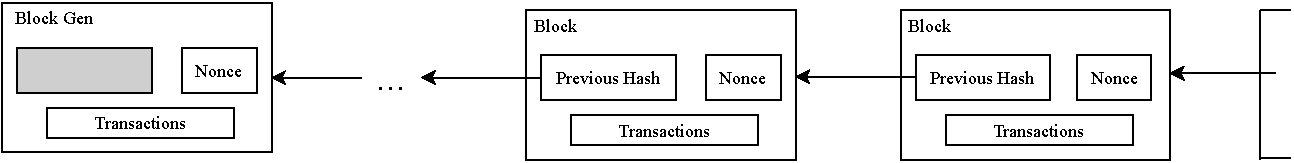
\includegraphics[scale=0.7]{figures/abstract_chain.pdf}
	\end{center}
	\caption{A high-level representation of a blockchain.}
	\label{fig:abstract_chain}
\end{figure}

A cryptocurrency blockchain is essentially a distributed ledger containing the history of the transactions made between the participating parties. The blockchain ledger has the following two fundamental properties: i) it is \emph{immutable} and, ii) it is \emph{append-only}. Sometimes separate blocks can be produced concurrently, creating a temporary fork. In addition to a secure hash-based history, any blockchain has a specified algorithm for scoring different versions of the history so that one with a higher score can be selected over others. Bitcoin uses a proof-of-work system, where the chain with the most cumulative proof-of-work is considered the valid one by the network. Peers supporting the ledger may have different versions of the history from time to time. They keep only the highest-scoring version of the database known to them. Whenever a peer receives a higher-scoring version (usually the old version with a single new block added) they extend or overwrite their own database and retransmit the improvement to their peers. There is never an absolute guarantee that any particular entry will remain in the best version of the history forever. Blockchains are typically built to add the score of new blocks onto old blocks and are given incentives to extend with new blocks rather than overwrite old blocks. Therefore, the probability of an entry becoming superseded decreases exponentially as more blocks are built on top of it, eventually becoming very low.

\subsection{Transactions}
The transactions in an electronic coin are defined as a chain of digital signatures. Each owner transfers coin value to the next owner by digitally signing a hash of the previous transaction and the public key of the next owner and adding these two to the end of the transaction script, which is publicly announced to the network. A payee can verify the signatures to verify the chain of ownership. Of course the payee should somehow verify that the value transferred is not double-spent by the owner without the trust of a third party authority. In the Bitcoin's Unspent-Transaction-Output \emph{(UTXO)} model each unspent coin value is included in the so-called UTXO set. Every peer inspecting the transactions in the network validates that the value transferred in a transaction $tx$ belongs in the current UTXO set before including $tx$ in a block. Each time that a peer updates its blockchain, he updates the UTXO set according to the new transaction history too. By agreeing on a single blockchain history according to the highest score (highest PoW score for Bitcoin) among the all the existing chains in the network, the peers can also agree on a single history as for the sequence of the transactions made so far.

\begin{figure}[h!]
	\begin{center}
		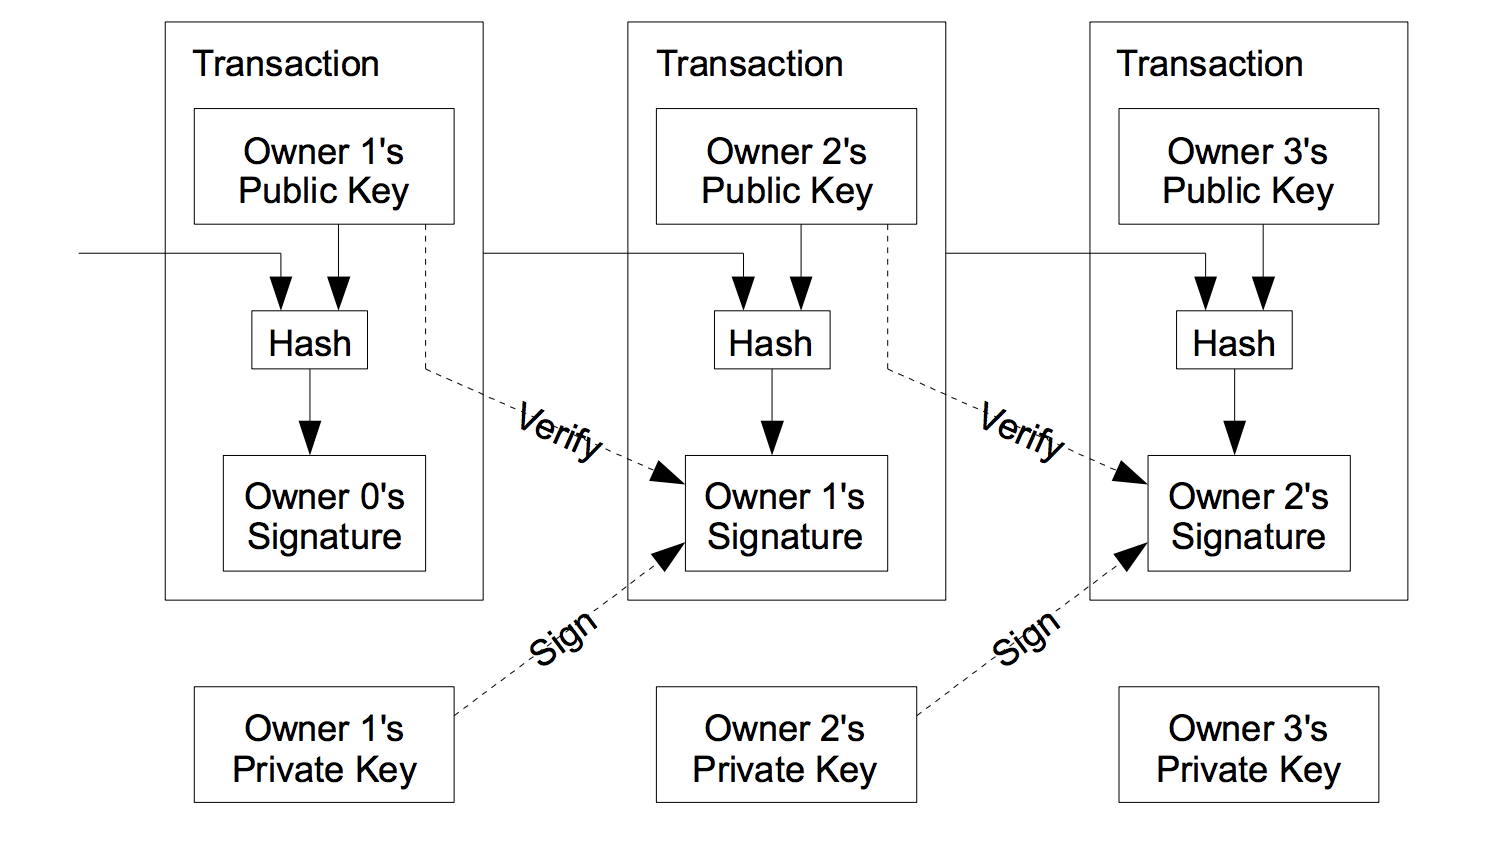
\includegraphics[scale=0.3]{figures/txs.png}
	\end{center}
	\caption{Transactions as a chain of digital signatures in Bitcoin~\cite{nakamoto}}
	\label{fig:txs_nakamoto}
\end{figure}


\subsection{The SPV model}
In the Bitcoin blockchain network each peer may have one of the following three roles: \textit{clients}, full \textit{nodes} and \textit{miners}. Miners maintain an updated copy of the chain locally, while providing computational power, also called hashpower, to extend it. In order to extend the chain by one block, the miner has to perform a proof-of-work as already described. Full nodes can be thought of as miners with zero hashpower. Full nodes are also called \textit{provers}, since they provide proofs  answering the queries for specific chain information made by clients.

In order to make the client functionality more efficient the Simple Payment Verification was proposed~\cite{nakamoto}. Based on the SPV scheme, there can be \emph{lightweight clients}, meaning clients that need to store only the block headers of the chain. A block header includes only a Merkle Tree Root of the Merkle Tree comprised by
the transactions included in that specific block. In order to validate that a transaction is
finalized, a client needs to query the nodes until he is convinced that he has the longest
valid chain, search for the block containing that transaction and finally verify an inclusion
proof of the transaction in the block of interest.

\begin{figure}[h!]
	\begin{center}
		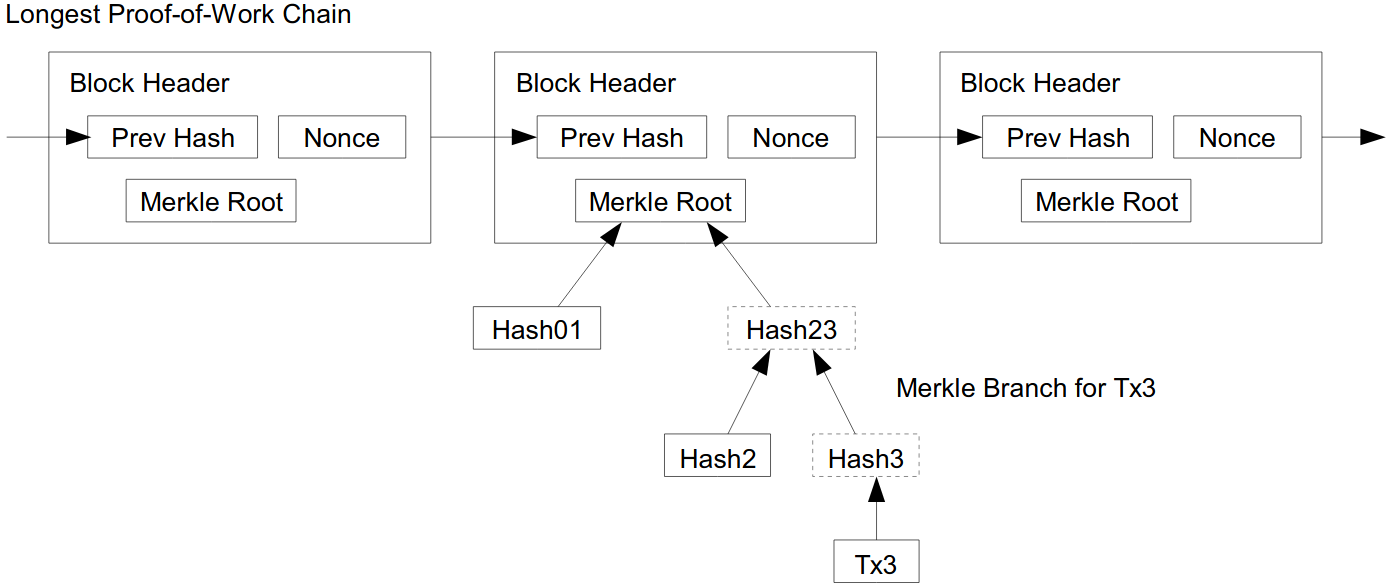
\includegraphics[scale=0.3]{figures/SPV_nakamoto.png}
	\end{center}
	\caption{High level representation of blockchain data kept by a lightweight client
	 and an inclusion proof for a transaction Tx3.\cite{nakamoto}}
	\label{fig:SPV_nakamoto}
\end{figure}

In the SPV scheme a client needs to store blockchain data of linear size to the whole chain. By
the time of writing Bitcoin's blockchain counts to almost 264GB and is estimated to grow more
than 50GB per year.  Since the growth of the chain is constantly increasing in a linear fashion, there is a need
to construct more efficient protocols serving the needs of lightweight clients. 
%Towards this end, the interaction between clients and full nodes is in our case supported  by the NIPoPoWs\cite{nipopows} primitive which allows polylogarithmic poofs to the size of the chain.